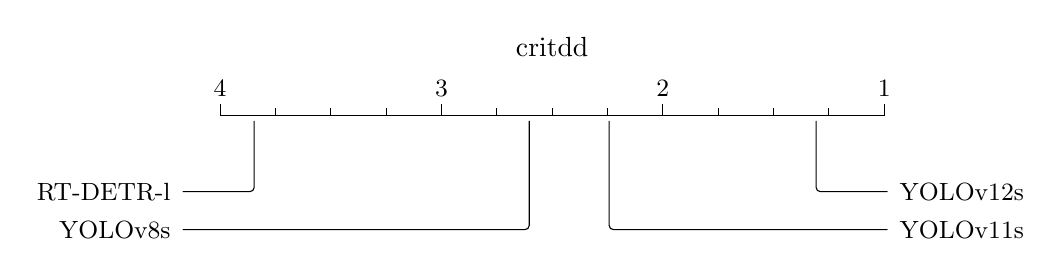
\begin{tikzpicture}[
  treatment line/.style={rounded corners=1.5pt, line cap=round, shorten >=1pt},
  treatment label/.style={font=\small},
  group line/.style={ultra thick},
]

\begin{axis}[
  clip={false},
  axis x line={center},
  axis y line={none},
  axis line style={-},
  xmin={1},
  ymax={0},
  scale only axis={true},
  width={\axisdefaultwidth},
  ticklabel style={anchor=south, yshift=1.3*\pgfkeysvalueof{/pgfplots/major tick length}, font=\small},
  every tick/.style={draw=black},
  major tick style={yshift=.5*\pgfkeysvalueof{/pgfplots/major tick length}},
  minor tick style={yshift=.5*\pgfkeysvalueof{/pgfplots/minor tick length}},
  title style={yshift=\baselineskip},
  xmax={4},
  ymin={-3.5},
  height={4\baselineskip},
  xtick={1,2,3,4},
  minor x tick num={3},
  x dir={reverse},
  title={critdd},
]

\draw[treatment line] ([yshift=-2pt] axis cs:1.3076923076923077, 0) |- (axis cs:0.9743589743589745, -2.0)
  node[treatment label, anchor=west] {YOLOv12s};
\draw[treatment line] ([yshift=-2pt] axis cs:2.242603550295858, 0) |- (axis cs:0.9743589743589745, -3.0)
  node[treatment label, anchor=west] {YOLOv11s};
\draw[treatment line] ([yshift=-2pt] axis cs:2.603550295857988, 0) |- (axis cs:4.17948717948718, -3.0)
  node[treatment label, anchor=east] {YOLOv8s};
\draw[treatment line] ([yshift=-2pt] axis cs:3.8461538461538463, 0) |- (axis cs:4.17948717948718, -2.0)
  node[treatment label, anchor=east] {RT-DETR-l};

\end{axis}
\end{tikzpicture}